\chapter{Introduction}
\section{Background and Motivation}
As the global demand for security and automation increases, many seek to use video anomaly detection systems. Leveraging modern computer vision, modern anomaly detection systems play an important role in increasing monitoring efficiency and reducing the need for expensive live monitoring. Their use cases can vary from detecting faulty products on an assembly line or detecting car incidents on the highway, and everything in between. In the US alone, the surveillance market is expected to reach $\$23.60$ Billion by 2027 \cite{us_video_stats}.
\par
The most important component in video anomaly detection systems is the intelligence behind it. The intelligence ranges from simple on-board algorithms to dedicated servers hosting complex deep learning models, where the latter has seen increased popularity the past few years.\par
\begin{figure}[H]
    \centering
    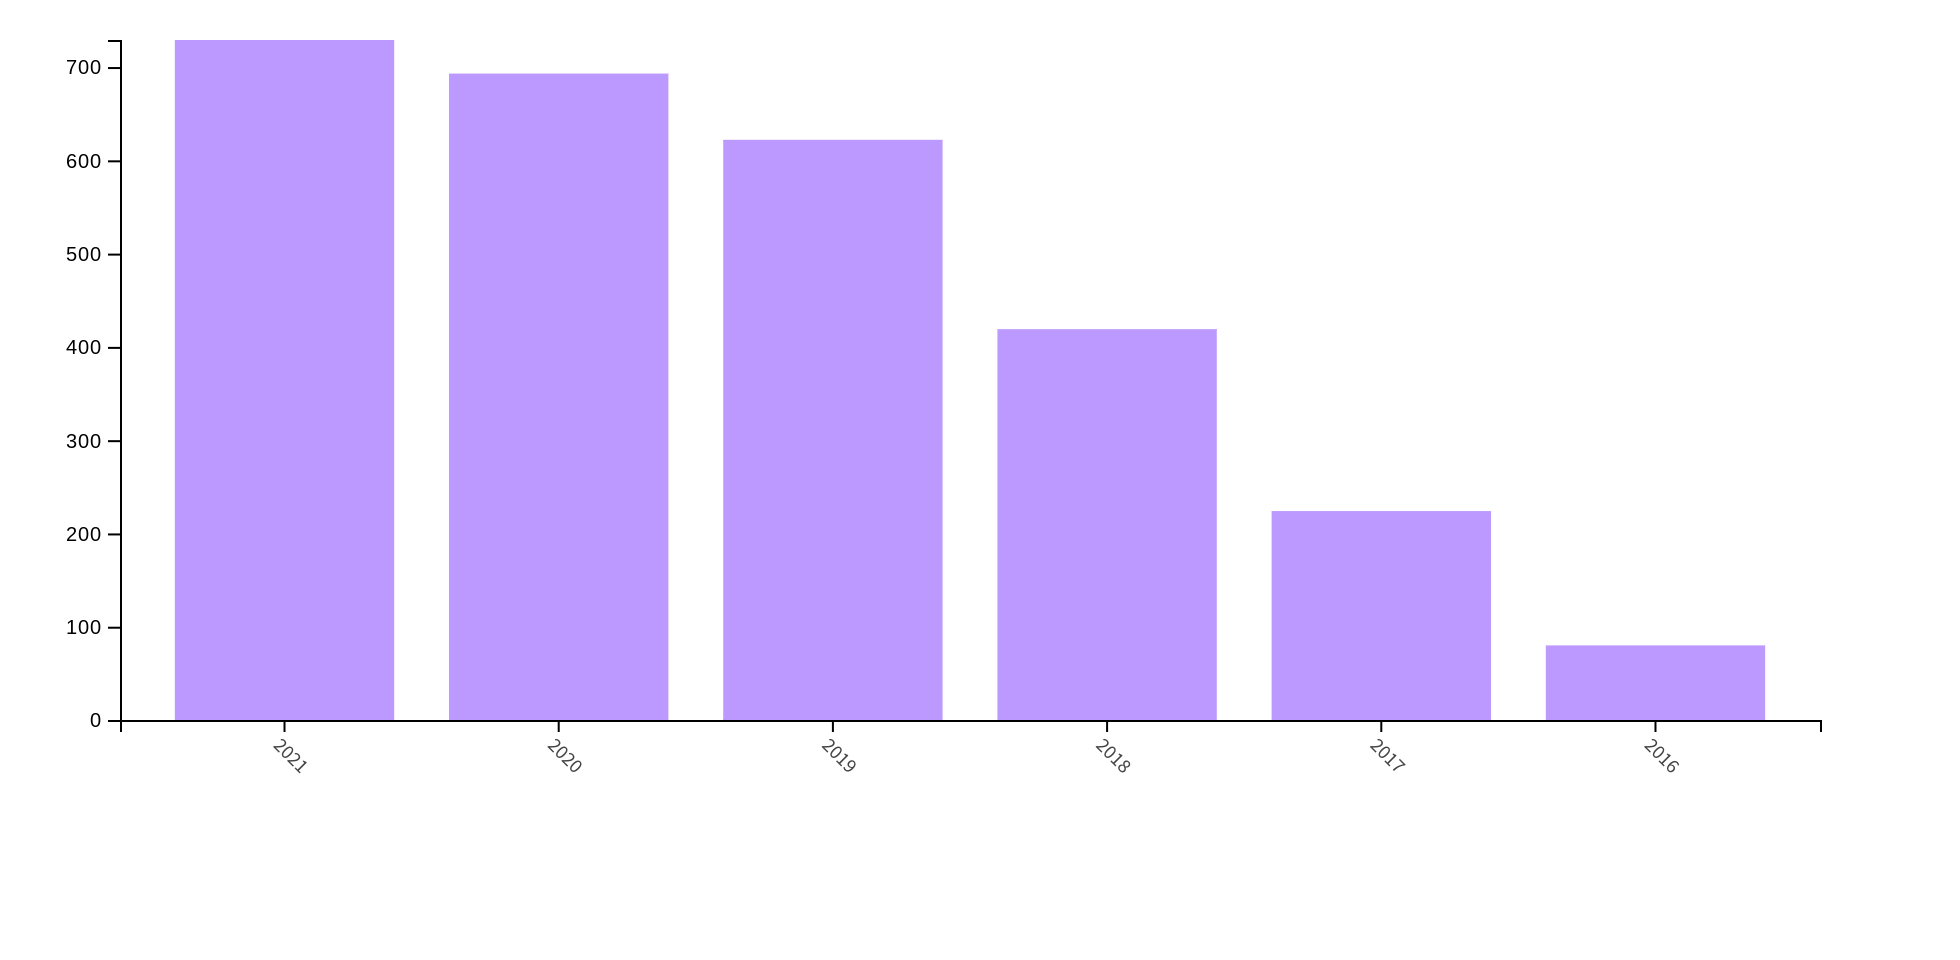
\includegraphics[width=\linewidth]{resources/introduction/deep_learning_surveillance_chart.jpg}
    \caption{The increase in publications mentioning the terms "deep learning" and "surveillance". \cite{deep_learning_surveillance_stats}}
\end{figure}
Yet despite the major progress within the field of deep learning, there are still many tasks where humans outperform models, especially in anomaly detection where the anomalies are often undefined. Deep learning approaches also perform poorly when dealing with noise and concept drift.
\par
The cause for the discrepancy lies in the difference between how humans and machine learning algorithms represent data and learn. Most machine learning algorithms use a dense representation of the data and apply back-propagation in order to learn. Human learning happens in the neocortex, where evidence points to that the neocortex uses a sparse representation and performs Hebbian-style learning. For the latter, there is a growing field of machine learning dedicated to replicating the inner mechanics of the neocortex, namely Hierarchical Temporal Memory (HTM) theory. This theory outlines its advantages over standard machine learning, such as noise-tolerance and the ability to adapt to changing data.
\par
With the advantages of HTM and the rise of video anomaly detection in mind, a natural question one could pose is whether it is possible to apply HTM for anomaly detection in videos. Combined with a lack of related works, it is this very question that is the motivation behind this thesis.
\section{Problem Statement}
Based on the background and motivation, the problem statement can be boiled down to a simple question: \textbf{Is HTM viable for use in video anomaly detection?}\par
This thesis will introduce three different experiments that will help answer the question and also showcase the performance of HTM. These experiments will vary in difficulty and complexity. This thesis will cover three objectives:
\begin{enumerate}
    \item Introduce HTM and give a deep understanding of the inner workings, the strengths, and the weaknesses. While also being friendly to readers with a machine learning background.
    \item Develop and outline a theoretically sound pipeline so that HTM can be applied for anomaly detection in complex videos.
    \item Perform experiments, discuss the results, and lay out potential future work.
\end{enumerate}
\section{Limitations}
HTM is a complex topic not part of the curriculum in most universities, if any at all. This makes learning and understanding HTM a process which takes up a sizable chunk out of the total time spent on the thesis. This thesis will  therefore mainly focus on only one approach, leaving other approaches for other papers.\par
In addition, HTM for video anomaly detection is a novel topic and is therefore naturally limited on several fronts. One of the main limitations is the lack of labeled anomaly data that suits the nature of HTM, because most datasets are made for use with deep learning approaches. Another problem is the lack of works related to applying HTM on video-based problems. Finally, there are no direct benchmarks that can be compared.
\section{Contributions}
This thesis contributes in multiple ways. Not only does it present a novel way to apply HTM to video-based problems, it also uncovers the reasoning behind the design decisions that were made as well as providing thorough analysis. This thesis also acts as an organization of HTM related research and ties it into deep learning.
Github contribution.
